\chapter{Digitizers, Crate Controllers, and Logic Modules, oh my!}\label{ch:hardware}

Much of this chapter deals with the intricacies and nuances of the CAEN V1724, but the general principles can be applied to other makes and models, provided the same principles hold.
The V1724 is not designed to do any on-board processing beyond its deadtime-free circular buffer and ZLE, unlike (for instance) the Skutek DDC10 that the HEV is built with.
We'll also discuss the other VME (and VME-adjacent) hardware.

\section{V1724}\label{sec:v1724}

This digitizer is the workhorse of the DAQ.
The TPC readout uses 62 for the main PMT channels, a further 32 for the high-energy channels, and a 95th as the acquisition monitor.
The muon veto uses 11 with the default firmware, and the neutron veto uses one.
While it is by and large very reliable, it has the occasional quirk.

First some things should be laid out for the sake of clarity.
There are a variety of options of firmwares available for the V1724, and we use different ones depending on the task.
The muon veto uses the default firmware without ZLE.
The TPC uses the DPP DAW (digital pulse processing, dynamic acquisition window) firmware, which is effectively ZLE on steroids.
The DPP DAW firmware allows for the independent triggering and readout of channels on a board, so you don't need any trigger logic above self-trigger thresholds.

\subsection{Timestamps}

Perhaps the most annoying limitation is its internal timestamp clock.
The V1724 timestamp clock runs at the same \SI{100}{\mega\hertz} as the ADC, but the on-board counter only has 31 bits.
This means that the clock will roll over every \SI{21.47483648}{\second}.
The V1730 has a 48-bit clock, so you can run that thing for days.
We don't have this luxury.
There are a few ways of dealing with this.
Running for only \SI{21.5}{\second} is technically an option, but no.

\subsubsection{Strict a $>$ b tracking}

The data you read from the digitizer is strictly time-ordered, so the ``absolute'' timestamp of event n+1 is going to be greater than that of event n, because that's how time works.
At some point the binary representation of this absolute timestamp hits the 32nd bit, and bits[0:31] roll back to 0.
If you track every timestamp, it should be pretty clear that you just recorded a timestamp less than the previous value.
Ergo, the clock just rolled, and you increment the rollover counter up by one.
When you reconstruct the ``absolute'' timestamp of this event, you add \texttt{rollover\_counter<<31} onto whatever value the digitizer returned.

\subsubsection{Progression tracking}

Alternately, some more convoluted logic can be employed.
You can watch the timestamps go from ``small'' (less than \SI{5}{\second} or so), to ``neither small nor large'', to ``large'' (at least \SI{15}{\second}), and then increment the rollover counter when you see the board go from ``large'' to ``small''.
This assumes you have enough data coming in so that you don't miss one of these steps.
If you do happen to miss one step (maybe you go from ``small'' straight to ``large''), you had better hope that you implemented logic that can handle this.
This technique is great if you do readout asynchronously, but this is difficult to do because optical links aren't thread-safe.
It is useful for the waveform simulator, though.

\subsubsection{Missed rollovers}

Suppose you don't see any data from a digitizer for more than one rollover cycle (maybe you have a \emph{really} low background detector).
You'll still see the clock rollover, but you've missed an entire cycle, so you're now off by \SI{21.5}{\second} in your timestamp reconstruction.
Figure~\ref{fig:digi_missed_rollover} will facilitate discussion.

\begin{figure}[h]
  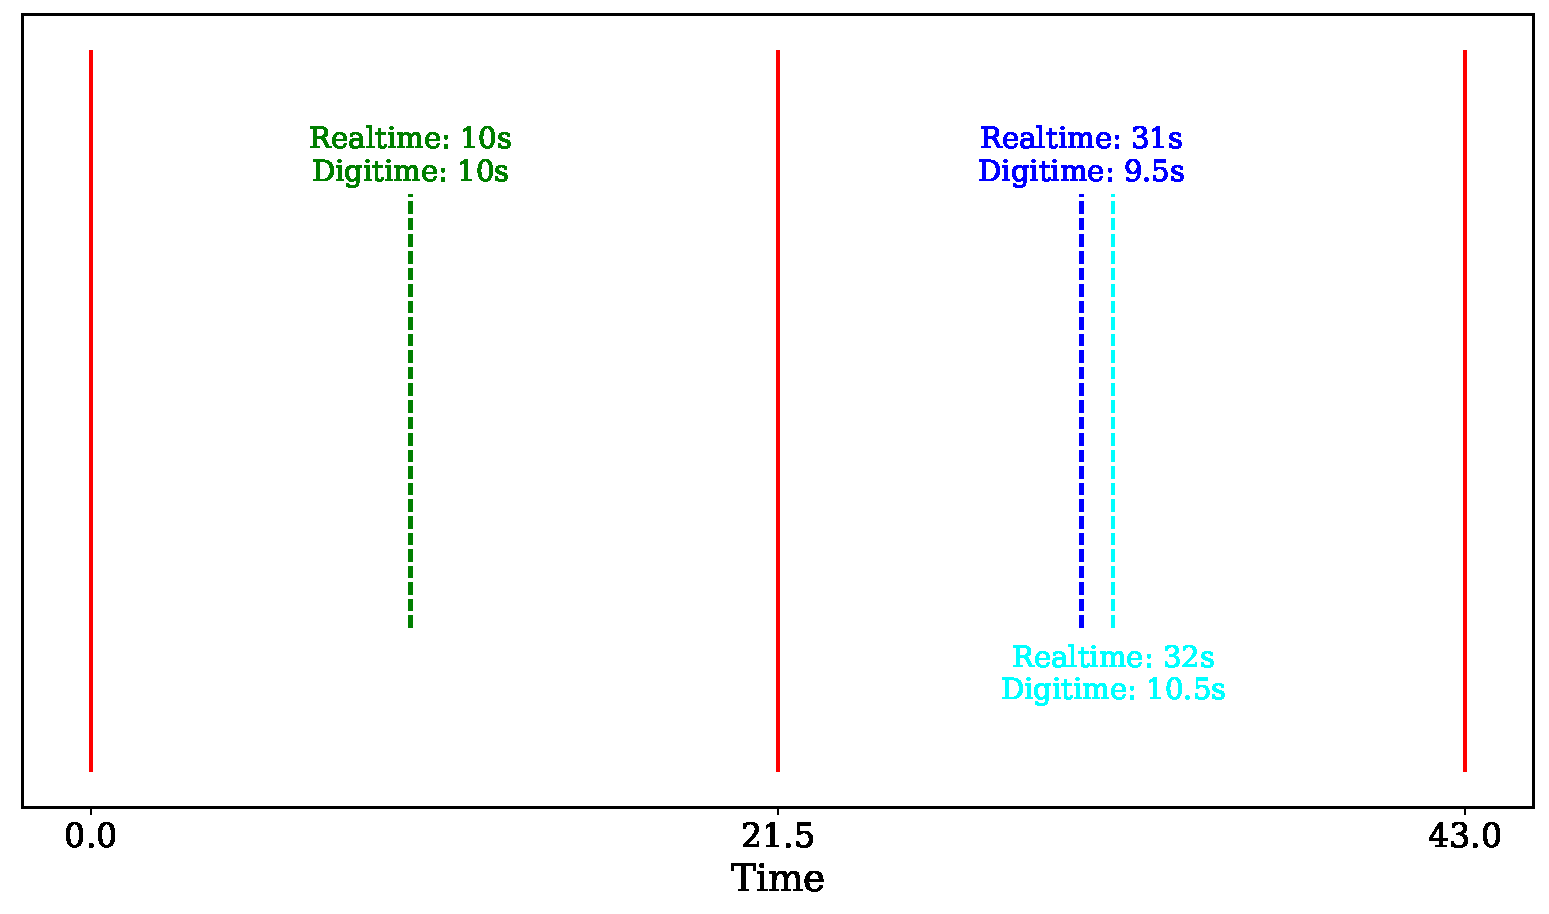
\includegraphics[width=\textwidth]{images/digitizers/missed_rollover}
  \caption{Missing digitizer rollover cycles}\label{fig:digi_missed_rollover}
\end{figure}

The green event comes along and gives us a digitizer timestamp.
If the next event we see is the blue event, we can see that its digitizer timestamp is less than the previous (green) value, so we acrue an additional rollover counter and all is well.
If, however, the next event we see is not blue but cyan, all is not well.
The cyan timestamp is greater than that of green, so no rollover has been observed.
With our perfect knowledge of realtime, we can easily see that a rollover was missed.

The simplest way to deal with this is to also track the unix timestamps of readouts.
If the unix timestamps differ by more than one cycle (such as for cyan), then you've missed one, so increment your counter as appropriate.
However, what if the blue timestamp was measured half a real second later?
Now we've just accrued an unwanted extra rollover, this board's data is \SI{21.5}{\second} ahead of where it should be, and the rest of that run's data is garbage.

It turns out (surprise surprise) that there's nuance involved.
What \emph{is} the realtime of a digitizer event?
We don't know exactly when acquisition started (not to the precision necessary, and the readers don't have access to this anyway).
We don't know the time delay between when the event was stored for readout in the digitizer, and when it actually gets read out.
If the optical link is under ``low'' load, then there is maybe a few microseconds between when an event is prepared for readout and when readout happens.
We use 8~MiB digitizers, which means in the worst case it could be nearly an entire second until the event is read in the worst case where all the other digitizers are totally full.
Either way, there will be some time difference.
The best solution is not to run without at least a Hz or so of something, or use an external trigger of some sort.
Worth pointing out here - if the boards are configured in self-trigger mode, any external trigger (be it the TRG-IN, a SW trigger, LVDS, etc) is ignored, so you can't implement logic to periodically poke these boards to make sure they return something.

\subsection{Crashes}

Digitizers are computers.
They sometimes crash.
They'll often do this in ways that don't make sense.

If the \SI{50}{\mega\hertz} clock signal becomes unstable or gets interrupted, you have maybe a few seconds before the board crashes.
Best to catch it, issue a stop command, and then a PLL reconfiguration.
If you don't catch it, boards start throwing -2 errors.

Sometimes the digitizer will return garbage data, and the readout software will probably segfault while dealing with it.
When programs segfault they usually don't do proper garbage collection and cleanup, which means the connection to the digitizer isn't closed correctly.
The next time the software tries to connect to the digitizer there's a good chance it'll refuse to connection.
To fix this you connect with another piece of software and reset the board.

\subsection{Sleep 2}

This was a magical line added to the readout software to prevent crashes.
For a long time we didn't know why this worked.
After you write to the reset register, the digitizer doesn't really respond properly for a second or so while it boots.
If you try to ask it to do something before it's finished booting, it might crash.
\texttt{sleep(2)}.
Magic.

\subsection{Baselining}

The trigger threshold for the default firmware is an absolute value, so making sure the baseline is set accurately is important.
The self-trigger firmware uses a relative threshold, so it's less important, but a poorly-set baseline still costs you dynamic range.
The baseline routine used to be the only consistent source of crashes.
Earlier versions of the baseline routine (see Section~\ref{sec:baseline}) tried to do a lot of things very quickly, and the boards seem to dislike this.
It's now a source of particularly rare segfaults, but this isn't a result of the digitizers.

\subsection{Clocks}\label{sec:digi_clocks}

I'll put this as a subsection rather than a section because the digitizers are the only thing that need clock inputs.
The board needs a \SI{50}{\mega\hertz} clock signal for the on-board electronics to function; this frequency will get stepped up to other necessary frequencies (like the \SI{100}{\mega\hertz} ADC and trigger clocks, and the \SI{1}{\giga\hertz} VCXO clock).
Every board has its own, but if you're running multiple you want them to drift together rather than individually.
Usually you implement this by having one board provide the master clock signal with its internal clock, and then just propagate this clock down the line of boards.
The catch is that this propagation of clocks is an analog copy-paste operation.
After 60 or 70 boards you've copy-pasted so much noise into the signal that you can no longer use it as a reference clock.
How, then, do you synchronize 120 boards?
One crate at a time, is the answer.
You use one external master clock with multiple outputs (we use the CAEN DT4700), and then run cables to the first board in each crate and then chain each crate together.
If each cable going from your master clock to the crates is the same length modulo the signal phase then the signals all arrive at the digitizers in-phase, and your synchronization is maintained.
This doesn't require that the cables be exactly the same length in usual distance units, rather that they are the same number of clock wavelengths in length.
It doesn't matter if some boards get a clock signal that's technically a few cycles older than another as long as they have the same phase, because it's a clock signal.

Worth also mentioning here, each board has a programmable delay that can be added to the output signal.
For a short clock cable about \SI{7}{\centi\meter} in length, the best delay we found was around \SI{3600}{\pico\second} with some variation between boards.
This ensures that all signals arriving at each digitizer have the same phase, so the boards all clock together properly.
Also, get your electronics workshop to make the cables, \emph{especially} the long ones.
They're better at it than you are, and shitty clock cables will cause a lot of crashes.
If there are instabilities in the clock signal the boards will crash.
If the cables are trash then jiggling them will cause some of these instabilities.
If the cables are trash then they'll probably pick up lots of noise, and this will cause some of these instabilities.

\section{V2718}\label{sec:v2718}

This piece of hardware is how we handle the synchronization of the S-IN signal, controlling whether or not we send various signals to things external to the TPC DAQ (specifically, whether the S-IN signal goes to either of the vetos, and if the external trigger is propagated to the LED pulser), and generating the external trigger.

The external trigger isn't all that convenient to work with.
It doesn't offer continuous frequencies, it's implemented via selecting a time unit (\SI{104}{\milli\second}, \SI{410}{\micro\second}, \SI{1.6}{\micro\second}, and \SI{25}{\nano\second}) and how many of them you want (1-0xFF).
This means that some frequency ranges are well-served but others have large gaps where no valid values exist.
The chances are good that at least one of the three frequencies you need (PMT gain, PMT AP, and noise) will fall into one of the regions where you only have a very few values.
You can also specify the width of the output pulse, but that doesn't matter much for us so it's always 1.

The V2718 also maintains its state after you disconnect from it - the status of any output signals will be held, so if a dirty shutdown happens you can sometimes end up with an orphaned S-IN where the signal is still high but you no longer have an active connection to the hardware.
When this happens you have to issue an ARM command to reestablish the connection, so when the STOP comes it'll reset the output.
Also, when it boots, it sometimes decides that it's going to put all of its outputs to 1?
Can't confirm, but this might be the cause of some issues we occasionally have.

\section{V1495}

This is described as a ``general-purpose programmable logic board''.
It's got a couple of user-programmable FPGAs and a variety of input types.
We use the large multi-channel ribbon cable LVDS inputs, hooked to the LVDS output of each digitizer.
This allows the V1495 to collect the BUSY status of all digitizers and issue vetoes when appropriate.
We also use the V1495 to output a periodic veto signal as a data-rate-control technique.
If Operations wants you to collect data when the water tank is empty, this is probably how you're going to do it.
For more details on the V1495 see Alexey's thesis.

There's a considerable amount of additional potential afforded by this module that we aren't really taking advantage of.
It does the trigger logic for the MV and the BUSY logic for the TPC, but that's about it.
I don't immediately have ideas for extensions because the nT paradigm is to get everything off of FPGA and into the servers as soon as possible, but I know there are further uses that we could exploit.
It's also worth pointing out that the V1495 is old, obscelete, and no longer in production.
It was superseded by the V2495 which uses a much more modern chip.

\section{DDC10}

This is one further use of FPGA that we use.
The Skutek DDC10 looks similar to the V1724 but we have access to the FPGA so we can run custom firmware on it.
We implemented the HEV using the DDC10.
This scans the input signal (the sum signal from the bottom PMTs) for large S2s and issues a veto signal if it identifies one.
This is really useful during calibration, because AmBe and radon calibration generates a large amount of high-energy events, and we know these aren't useful for analysis.
If you prevent the digitizers from even recording these events you significantly reduce the overall rate (making Computing happy) and also enable calibration at a higher overall rate (unless your detector is broken and pileup is a much more significant issue).

The trickiest part of what this module does is the calculation of shape parameters of the incoming peaks.
S1s are too narrow for the current algorithm, the calculation is too slow and the peak is long gone by the time we're able to decide it was ever there.
Also, the easiest way to calculate the shape of a peak is to be able to look at the whole waveform, but this then requires that you can buffer the whole thing.
This is easier said than done.
I don't know enough about FPGA design to talk about dynamic memory allocation like I can for a modern CPU.
Also remember that this is an FPGA so you don't really have access to floating-point operations in the same way as on a CPU.
I feel that there is significant room for improvement in how these algorithms work, but again, we aren't FPGA masters.
For more details see Alexey's thesis.
